%
% !TeX root = ../letter.tex
% !TeX spellcheck = en_GB
%

\begin{ReviewerComment}
The manuscript presents an ambitious framework that integrates surrogate modeling and deep reinforcement learning for urban morphology and energy optimization. However, several critical issues currently limit the robustness and interpretability of the reported findings. Substantial changes are required before the manuscript can be considered for publication.
\end{ReviewerComment}
%
\begin{Answer}
We sincerely thank the Reviewer for the careful reading and for the constructive and technically demanding comments. We agree that the earlier manuscript framed the optimizer comparison too optimistically and did not communicate the methodological limits of the current evidence with sufficient clarity. We therefore used these comments to rethink not only individual paragraphs, but the overall presentation of the paper. The revised paper is no longer presented as a DRL-superiority study. Instead, it is framed as a surrogate-conditioned benchmark-fragility study in which the selected 2000-sample surrogate, the checkpoint-sensitivity audit, the same-budget CMA-ES follow-up, the independent candidate reevaluation, and the bounded physical probe are used together to support a more cautious interpretation. We respond point by point below.

In practical terms, this revision is not a light editorial cleanup. We revised the title, abstract, contribution list, benchmark section, discussion, and conclusion; rebuilt the main benchmark figure set; expanded Appendix~A with scale-study and surrogate-fidelity diagnostics; expanded Appendix~B with checkpoint-sensitivity, independent reevaluation, and bounded physical-probe evidence; and systematically corrected notation, figure labels, captions, units, and abbreviation handling. Our intent in the present response letter is therefore to make these changes visible rather than simply state that the manuscript has been revised.
\end{Answer}

\begin{ReviewerComment}
1. The study relies exclusively on simulated outputs to generate the dataset for surrogate modeling and DRL optimization, without any empirical or independent external validation to assess the realism of the simulation results.
\end{ReviewerComment}
%
\begin{Answer}
We agree that full empirical or full-stack external validation is still unavailable, and we now state that limitation explicitly. At the same time, the revision strengthens the validation side in two bounded ways.

First, Appendix~B now reports an independent deterministic reevaluation of the selected DDPG and NSGA-II candidates, so the final comparison is no longer interpreted solely through optimization-time surrogate predictions.

Second, we added a small-batch physical probe on representative candidates. Under the current best-aligned project workflow, EUIt shows the strongest agreement, EG remains a simplified but directionally stable proxy, and H is now checked through a January~20 windowsill-style direct-sun-hours workflow that is much closer to the manuscript definition than the earlier proxy. We also state explicitly that this does not constitute full physical closure.

Accordingly, the point is addressed through stronger bounded validation and much clearer framing, but not by claiming that external validation is fully closed. We appreciate this criticism because it helped us avoid presenting the revised package as more complete than it really is.
\end{Answer}
\begin{RevisionExcerpt}
\noindent\textbf{Revised evidence-scope text:}\\
``The benchmark comparison is conducted on the selected 2000-sample surrogate derived from the analytic response-generation workflow, whereas direct physical probing is currently available only for a small set of representative candidates. The results below therefore combine a full surrogate-space benchmark with a bounded physical cross-check rather than a fully symmetric end-to-end physical rerun.''\\[0.5em]
\noindent\textbf{Revised abstract text:}\\
``A small-batch physical probe adds bounded external support: EUIt aligns most consistently, the current EG check remains weaker but directionally stable, and a revised windowsill-style direct-sun-hours check places H in the same broad range as the surrogate values, albeit with weaker stability than EUIt.''
\end{RevisionExcerpt}
\begin{center}
\begin{tabular}{lccc}
\hline
Representative candidate & EUIt & EG & H \\
\hline
DDPG / balanced (surrogate) & 66.000 & 2.850 & 7.850 \\
DDPG / balanced (physical probe) & 74.379 & 2.637 & 7.525 \\
NSGA-II (surrogate) & 69.443 & 2.613 & 7.569 \\
NSGA-II (physical probe) & 74.057 & 2.828 & 6.075 \\
\hline
\end{tabular}

\vspace{0.4em}
\footnotesize Representative values summarized from the bounded physical probe now reported in Appendix~B.
\end{center}
\begin{center}
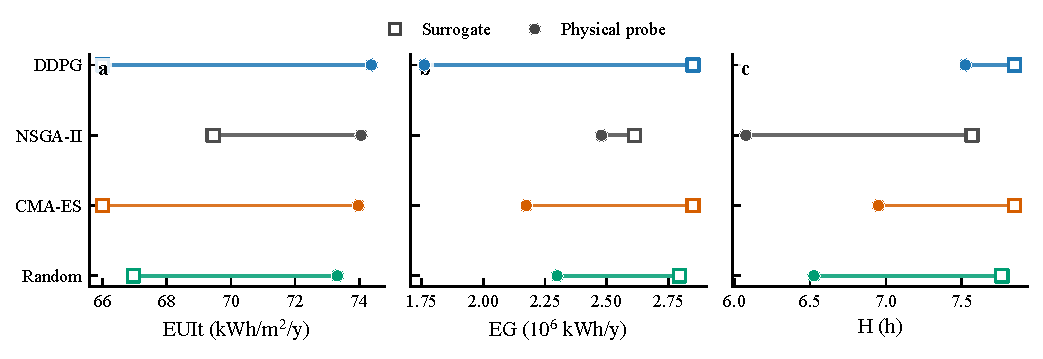
\includegraphics[width=0.80\linewidth]{../elsarticle/fig13.pdf}

\footnotesize Revised four-method physical-probe figure included in Appendix~B to make the new validation-mode evidence directly visible.
\end{center}

\begin{ReviewerComment}
2. The claimed superiority of the DRL framework over NSGA-II may be methodologically biased, as the utopian-point-based reward explicitly guides the search toward a predefined ideal region, whereas NSGA-II follows a standard Pareto-based formulation emphasizing diversity.
\end{ReviewerComment}
%
\begin{Answer}
We agree, and this concern is now treated as part of the paper's central interpretation. In the revised manuscript, the reward is described explicitly as a scalarized weighted-distance objective around a utopian point, not as a direct Pareto-learning formulation. We also removed the earlier superiority claim. On the selected highest-accuracy 2000-sample surrogate, fair-budget NSGA-II remains stronger than all three DDPG scenarios in objective summaries, Hypervolume, IGD, and preference-aligned utility. The DDPG scenarios are retained as evidence of preference-conditioned search bias on a surrogate checkpoint, not as proof of Pareto superiority.

To make this shift visible rather than merely verbal, the revised manuscript now reports the benchmark ordering directly through the main benchmark table and figure set. In particular, Table~\ref{paper:tab:perf} and Fig.~\ref{paper:fig:matched-benchmark} show that NSGA-II remains strongest on the selected surrogate, while the DDPG scenarios remain weaker and partially overlapping. We also added the main-text budget-accounting table so that the comparison protocol is explicit rather than implicit. This comment helped us replace a defensively framed response with a clearer statement of what the benchmark actually shows.
\end{Answer}
\begin{RevisionExcerpt}
\noindent\textbf{Revised contribution text:}\\
``This study shows that, on the selected highest-accuracy surrogate, fair-budget NSGA-II remains stronger than all three DDPG scenarios in archive-level Pareto metrics and preference-aligned utility, while the DDPG runs retain substantial late-stage instability.''\\[0.5em]
\noindent\textbf{Revised benchmark text:}\\
``Rather than claiming superiority of DRL over NSGA-II, the available evidence indicates that DDPG does not match fair-budget NSGA-II on the selected surrogate.''
\end{RevisionExcerpt}
\begin{center}
\begin{tabular}{lcc}
\hline
Method & HV & IGD \\
\hline
NSGA-II & 1.3310 & 0.1068 \\
Balanced DDPG & 0.3474 & 0.7196 \\
Saving DDPG & 0.6252 & 0.5491 \\
Generation DDPG & 1.0107 & 0.2205 \\
\hline
\end{tabular}

\vspace{0.4em}
\footnotesize Main benchmark numbers now reported in the revised manuscript for the selected 2000-sample surrogate.
\end{center}
\begin{center}
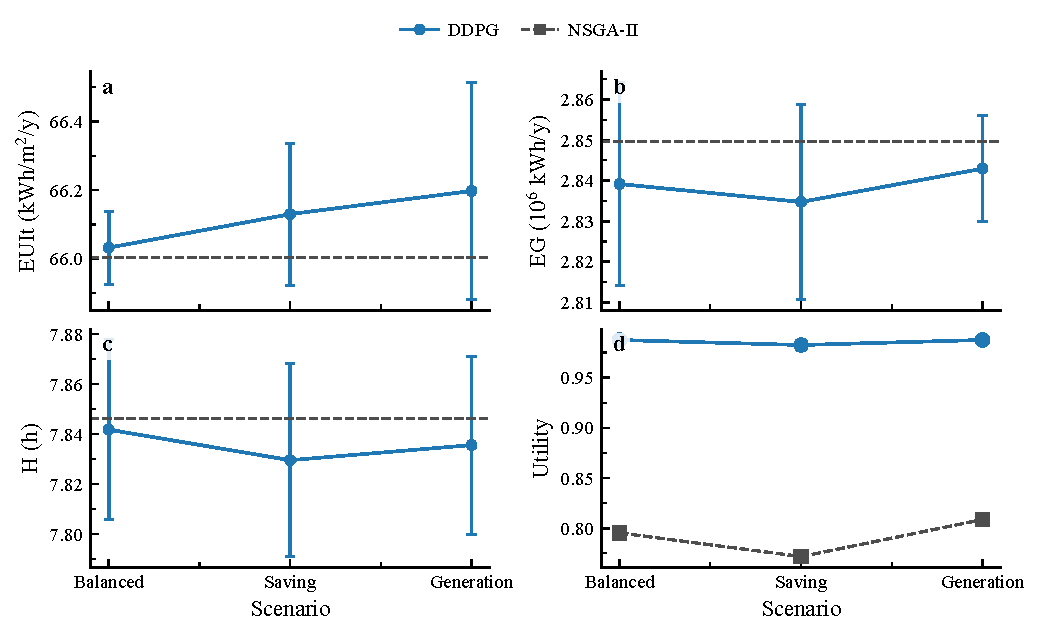
\includegraphics[width=0.80\linewidth]{../elsarticle/fig9.pdf}

\footnotesize Revised benchmark summary figure showing scenario-wise objective summaries and preference-aligned utility under the selected 2000-sample surrogate.
\end{center}

\begin{ReviewerComment}
3. The surrogate model is trained on only 500 samples in a 12-dimensional continuous design space, which may be sufficient for regression but is likely insufficient to robustly support surrogate-guided reinforcement learning optimization, particularly in extreme or sparsely sampled regions.
\end{ReviewerComment}
%
\begin{Answer}
We agree that the original presentation did not make the dataset scale and its implications sufficiently clear. The revised manuscript now distinguishes between the initial 500-sample baseline and the expanded 500/1000/1500/2000-sample scale study. The final optimizer benchmark is conducted on the selected 2000-sample surrogate, and Appendix~A now reports the scale-study diagnostics, cross-validation summary, and extreme-region error diagnostics together. We also retained an explicit limitation stating that even the selected 2000-sample surrogate still approximates a 12-dimensional continuous design space and should not be interpreted as closing extrapolation risk in sparse or extreme regions.

This change is also reflected in the current figure set. The revised manuscript no longer asks the reader to accept the final surrogate by default. Instead, the scale-study figure makes clear why the selected 2000-sample surrogate was retained for the final comparison and how the final benchmark is tied to an explicit model-selection procedure. This was an important improvement because the earlier draft left too much of that selection logic implicit.
\end{Answer}
\begin{RevisionExcerpt}
\noindent\textbf{Revised methodology text:}\\
``A dataset-scale study was carried out over 500, 1000, 1500, and 2000 morphologies, and the final optimizer comparison uses the most accurate surrogate identified from that study.''\\[0.5em]
\noindent\textbf{Revised limitation text:}\\
``Even with 2000 simulated cases, the surrogate still approximates a 12-dimensional continuous design space and therefore remains vulnerable in sparse or extreme regions.''
\end{RevisionExcerpt}
\begin{center}
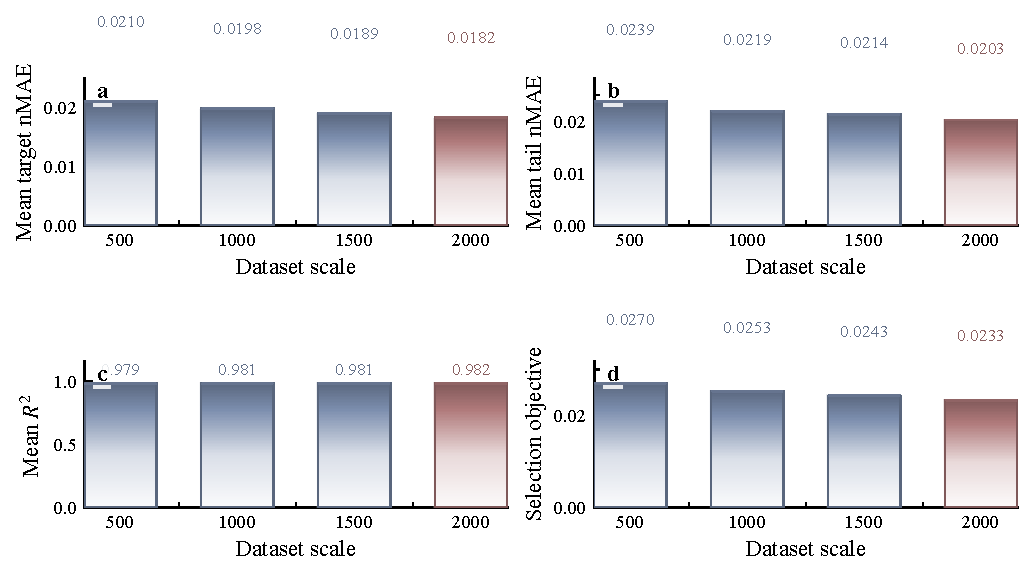
\includegraphics[width=0.78\linewidth]{../elsarticle/fig11.pdf}

\footnotesize Scale-study diagnostic figure now included in the manuscript to make the final surrogate selection traceable across the 500/1000/1500/2000-sample regimes.
\end{center}

\begin{ReviewerComment}
4. The literature review remains largely descriptive and lacks critical synthesis from an energy systems perspective, framing the research gap primarily as an algorithmic improvement rather than addressing unresolved challenges in energy system design and decarbonization.
\end{ReviewerComment}
%
\begin{Answer}
We agree and revised the Introduction accordingly. The current version now links the methodological contribution more directly to block-scale urban-energy design under decarbonization constraints and to the practical role of surrogate-assisted optimization as a screening layer before full physical validation. This allows the research gap to be stated as a domain-relevant methodological question: when optimization is surrogate-conditioned, benchmark reliability itself becomes part of the urban-energy design problem.
\end{Answer}
\begin{RevisionExcerpt}
\noindent\textbf{Revised Introduction text:}\\
``Large comparative sweeps over urban-energy design strategies are often bottlenecked by expensive simulation workflows, so surrogate-assisted optimization is increasingly used as a screening layer before full physical validation. However, once the benchmark itself is surrogate-conditioned, optimizer reliability becomes part of the research problem: if a learning-based method is unstable, checkpoint-sensitive, or difficult to compare fairly, its practical value for urban energy design remains uncertain.''
\end{RevisionExcerpt}

\begin{ReviewerComment}
5. On Page 17 (Line 55), the manuscript claims that the objective space contains complex, nonlinear valleys of high performance. However, the analysis presented on Pages 16-17 considers only linear relationships (Pearson Correlation). The absence of nonlinear interaction analysis is not adequately explained.
\end{ReviewerComment}
%
\begin{Answer}
We agree that the earlier wording was too strong. We removed the unsupported ``nonlinear valleys'' claim from the main text. In the revised manuscript, the correlation analysis is used only as a first-order interpretive tool, while nonlinear response information is reported in Appendix~B as supporting surrogate-based diagnostics. This narrows the claim to what is actually shown by the available evidence.
\end{Answer}
\begin{RevisionExcerpt}
\noindent\textbf{Revised appendix text:}\\
``To complement the linear correlation results in the main text, the appendix now reports representative surrogate-based nonlinear response profiles for OSR$\rightarrow$EUIt, FAR$\rightarrow$EG, SVF$\rightarrow$H, and $\theta\rightarrow$H.''\\[0.5em]
\noindent The stronger ``nonlinear valleys'' wording has been removed from the main manuscript.
\end{RevisionExcerpt}

\begin{ReviewerComment}
6. Given the 12-dimensional continuous action space, the training duration (200 episodes $\times$ 40 steps) appears relatively short. Stronger evidence or justification is required to demonstrate that the DRL agents have adequately converged.
\end{ReviewerComment}
%
\begin{Answer}
We agree. The final manuscript no longer relies on the earlier short-horizon presentation. Instead, the current training-dynamics evidence comes from guarded 600-episode multi-seed reruns with 20 seeds per scenario. More importantly, we no longer claim stable asymptotic convergence. The revised interpretation is intentionally narrower: policy learning can reach high-performing surrogate regions, but late-stage regression remains frequent, so the role of DDPG in the paper is diagnostic rather than as evidence of robust convergence to a final optimum.

To make this interpretation concrete, the revised text now reports the approximate plateau episodes together with the best-to-final reward gap ratios and substantial-regression fractions. On the selected 2000-sample surrogate, the 20-episode rolling reward reaches 95\% of its best observed value around episodes 401, 320, and 398 for the balanced, saving-focused, and generation-focused scenarios, respectively. However, the substantial-regression fractions remain high at 95\%, 85\%, and 100\%, which is why the revised manuscript no longer treats these runs as evidence of clean asymptotic convergence.
\end{Answer}
\begin{RevisionExcerpt}
\noindent\textbf{Revised training-dynamics text:}\\
``On the selected 2000-sample surrogate, seed-level diagnostics show that the 20-episode rolling reward typically reaches 95\% of its best observed value around episodes 401, 320, and 398 for the balanced, saving-focused, and generation-focused scenarios, respectively. At the same time, late-stage regression remains common, with mean best-to-final reward gap ratios around 0.62, 0.71, and 0.71 and substantial-regression fractions of 95\%, 85\%, and 100\% across the three scenarios. These curves therefore support a narrower interpretation: policy learning can reach high-performing surrogate regions, but it does not exhibit stable asymptotic convergence in this setting.''
\end{RevisionExcerpt}

\begin{ReviewerComment}
7. The manuscript title does not sufficiently convey the methodological advantage of the proposed approach over conventional NSGA-II-based optimization, despite this comparison being central to the paper's claimed contribution.
\end{ReviewerComment}
%
\begin{Answer}
We addressed this concern by changing the title in a more accurate and more conservative direction. Because the revised evidence does not support an optimizer-superiority claim, the new title foregrounds the methodological issue that the final paper actually supports, namely benchmark fragility under surrogate conditioning.
\end{Answer}
\begin{RevisionExcerpt}
\noindent\textbf{Revised title:}\\
``Surrogate-Conditioned Benchmark Fragility in Block-Scale Urban Energy Design: A Comparative Study of Policy Learning and NSGA-II''
\end{RevisionExcerpt}

\begin{ReviewerComment}
8. The graphical abstract is of insufficient resolution and does not meet the journal's publication standards.
\end{ReviewerComment}
%
\begin{Answer}
We thank the Reviewer for pointing this out. The graphical abstract has been replaced with a higher-resolution publication-quality version aligned with the revised manuscript framing.

In revising this asset, we also made sure that the graphical abstract is consistent with the current final message of the paper. In other words, the replacement was not only a technical export at higher resolution; the content shown in the graphical abstract was also aligned with the revised benchmark-fragility framing so that the visual summary does not continue to imply a stronger optimizer-superiority claim than the revised manuscript supports.
\end{Answer}

\begin{ReviewerComment}
9. The definitions of AF and OSR on Page 6 (Lines 45-46) are inconsistent with those in Supplementary Material S-1, which may cause confusion.
\end{ReviewerComment}
%
\begin{Answer}
We thank the Reviewer for noting this inconsistency. It has now been corrected. The definitions of AF and OSR are synchronized between the main manuscript and Appendix~A, where the former supplementary material has been consolidated.

We agree that such notation drift can undermine reader confidence, especially in a paper that already contains multiple objectives, multiple morphology descriptors, and several layers of appendix material. For that reason, we did not treat this as an isolated wording fix. Instead, we rechecked the morphology-factor definitions across the main text and appendix together and kept only one final definition for each quantity in the revised package.
\end{Answer}
\begin{RevisionExcerpt}
\noindent\textbf{Revision summary:}\\
The morphology-factor definitions in the main text and Appendix~A were checked and aligned so that AF and OSR now use one consistent definition throughout the revised package.
\end{RevisionExcerpt}

\begin{ReviewerComment}
10. Several formatting problems are present, including inconsistent or incorrect presentation of "$R^2$" on Page 6 and in Supplementary Material S-2.
\end{ReviewerComment}
%
\begin{Answer}
We thank the Reviewer for pointing out these formatting inconsistencies. This has now been corrected. The notation for $R^2$ is standardized in the main manuscript and Appendix~A, including the cross-validation and surrogate-fidelity tables.

More broadly, this correction was made as part of a systematic pass over notation consistency rather than as a one-line patch. During this pass, we checked the formatting of statistical symbols, table headers, and metric names together so that the validation-related tables now read as one coherent package.
\end{Answer}
\begin{RevisionExcerpt}
\noindent\textbf{Examples of revised headings:}\\
``Objective \& Mean $R^2$ \& Mean MAE \& Std.\ $R^2$ \& Std.\ MAE''\\
``Target \& RMSE \& MAE \& nRMSE \& MAPE (\%) \& $R^2$''
\end{RevisionExcerpt}

\begin{ReviewerComment}
11. A table in Supplementary Material S-2 (apparently corresponding to Table V) lacks a table title or caption.
\end{ReviewerComment}
%
\begin{Answer}
We thank the Reviewer for this observation. In the revised appendix, all retained tables now have explicit captions, including the surrogate-validation, checkpoint-audit, reevaluation, and physical-probe tables.

We agree that explicit captions are particularly important here because the revised appendix now carries a substantial portion of the technical evidence package. For that reason, we rewrote the captions so that they do not merely name the table, but also indicate what kind of evidence is being reported and how that evidence should be interpreted in the context of the revised manuscript.
\end{Answer}
\begin{RevisionExcerpt}
\noindent\textbf{Examples of revised captions:}\\
``Additional surrogate-fidelity audit on the cross-validation predictions of the selected 2000-sample surrogate.''\\
``Checkpoint-sensitivity audit for two 2000-sample surrogate checkpoints.''\\
``Independent re-evaluation of selected candidates from the highest-accuracy 2000-sample surrogate rerun.''
\end{RevisionExcerpt}

\begin{ReviewerComment}
12. Multiple figures and tables lack proper axis labels, units, or legends. In particular, Fig. 7 lacks y-axis explanations and units; Fig. 8, Fig. 11, Fig. 12, and Table VI lack units; Fig. 9 contains partially obscured indicators and missing units; Fig. 13 lacks axis labels and units in some subplots. The relationship between the upper and lower parts of Fig. 2 is unclear and should be clarified in the caption, and Fig. 3 requires clear explanations of colors and line types.
\end{ReviewerComment}
%
\begin{Answer}
We have revised the figure and table presentation substantially. Axis labels, units, legends, and caption explanations were checked systematically against the current final figure set. In particular, the benchmark, seed-diagnostics, scale-study, checkpoint-sensitivity, and physical-probe figures now use explicit units and revised captions consistent with the final selected-2000-sample narrative. We also clarified the workflow relation in the caption of Fig.~2 and updated the captions so that readers can interpret each panel without relying on the earlier supplementary package.

This revision required more than cosmetic relabeling. Because the paper's interpretation changed materially during revision, the figure set also had to be rebuilt so that the visuals matched the final evidence hierarchy. In practice, this meant revising panel labels, legend wording, unit annotations, and caption logic across the benchmark, diagnostics, and validation figures, rather than simply patching one or two isolated omissions.
\end{Answer}
\begin{RevisionExcerpt}
\noindent\textbf{Representative revised captions:}\\
``Comparison across fair-budget NSGA-II and the three DDPG scenarios on the selected 2000-sample surrogate.''\\[0.4em]
``Seed-level convergence diagnostics on the selected 2000-sample surrogate. Panels report the mean best reward, mean final reward, mean plateau episode, and late-regression fraction across 20 seeds per DDPG scenario.''\\[0.4em]
``Four-method small-batch comparison between surrogate predictions and the current best-aligned physical probe. Each row shows one representative candidate for DDPG, NSGA-II, CMA-ES, and RandomSearch, with square markers for surrogate values and circular markers for physical-probe values.''
\end{RevisionExcerpt}
\begin{center}
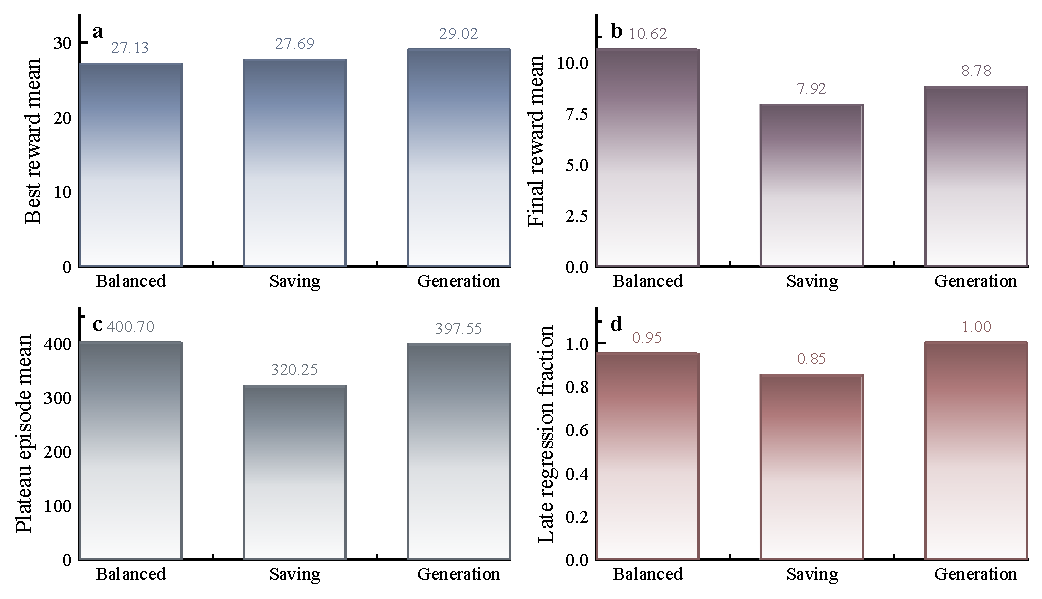
\includegraphics[width=0.78\linewidth]{../elsarticle/fig10.pdf}

\footnotesize Example of the revised diagnostic figure set, now presented with clearer panel structure, units, and caption support for the selected 2000-sample narrative.
\end{center}

\begin{ReviewerComment}
13. The manuscript does not include a list of abbreviations, which would improve readability given the extensive use of acronyms.
\end{ReviewerComment}
%
\begin{Answer}
We agree with this suggestion. An abbreviations list has now been added near the beginning of the manuscript in order to improve readability.

We found this addition particularly useful after the manuscript was revised into a more diagnostics-heavy version, because the current paper now refers repeatedly to UMFs, EPIs, DDPG, NSGA-II, CMA-ES, HV, IGD, and related terms across the main text and appendix. The abbreviations list is therefore intended not only as a formatting improvement, but also as a practical aid for readability.
\end{Answer}
\begin{RevisionExcerpt}
\noindent\textbf{Revision summary:}\\
The revised manuscript now includes an ``Abbreviations'' section listing the main acronyms used in the paper, including UM, UMF, EPI, MOO, DRL, DNN, DDPG, NSGA-II, CMA-ES, SAC, HV, and IGD.
\end{RevisionExcerpt}

\begin{ReviewerComment}
14. There are also several formatting issues on Page 6, such as "environments17" and "grid18", which should be corrected.
\end{ReviewerComment}
%
\begin{Answer}
We thank the Reviewer for identifying these issues. These spacing and merged-word artifacts have been corrected during the source-level revision of the manuscript. The current version no longer relies on the problematic imported fragments that produced those glitches.

To avoid leaving similar artifacts elsewhere, we did not treat these examples as isolated typos. Instead, we performed a broader source-level cleanup pass on the manuscript so that spacing, merged words, notation rendering, and local text-formatting problems were corrected together.
\end{Answer}
